\documentclass{article}
\usepackage[utf8]{inputenc}
\usepackage{color}
\usepackage{listings}
\usepackage{graphicx}
%\newcommand{\ahmad}[2][inline]{\color{orange} [Ahmad]: #2\color{black}}
\newcommand{\comm}[2][inline]{\color{red} #2 \color{black}}
\title{Capstone Project: TADA: a TAbular DAta classification of soft clusters using the Semantic Web}
\author{Ahmad Alobaid}
\date{\today}
 
\renewcommand*\contentsname{Content}
 
\begin{document}
 
\maketitle
 
\tableofcontents

\clearpage
\section{Definition (1-2 pages)}

\subsection{Project Overview}
In this century, people are storing and gather data more than ever in human history. We have massive amount of data scattered in different places. Before computers, information are kept in books and people used to look for information in the library, were a lot of books are kept. Today, we use search engines to look for information. According to \cite{webtables-power-2008} there are 154M tabular data they found in the web. Search Engines are performing quite well in finding textual data kept in webpages. But until today, search engine does not perform well when it comes to tabular data. They treat tabular data as textual data without taking into account the semantics hidden in the tables.

What we want to achieve is learning what does these data represents. Given enough data, we can deduce what a particular set of data represents, in other words, learns the type of this data. For example if you have the temperature for all the European countries, we will be able to tell that it is of the same type as set of temperatures of countries located in the American continent, both are temperatures of countries . Another example would be salaries for employees in Spain, we will be able to know that a set of numbers (e.g. salaries for employees in France) represent the salaries for employees. 

To reach this kind of learning that is done by computers, we use \textit{Semantic Web} to get data and their meaning, \textit{Machine Learning} for the learning process and statistical tests to be used by machine learning to distinguish a set of data from another. We will be focusing on numerical data, but this work can be extended to include categorical and textual data. In this work, we will not consider the relation between columns, but that can be an extension to the work. 

\comm{I might need to talk about data integration here}

\subsection{Problem Statement}
It is common for tables have missing headers, or headers that can\rq t be used as mentioned in \cite{webtables-power-2008} (e.g. if a column has the header "from", we don\rq t know if it is a time (a bus timetable) or a location (manufacturing countries)). So, we will be relying on the data in the column regardless of the header. 

Data Integration is also a common problem. Integrating multiple data sources can be a cumbersome as each data source can be in a different format. In the semantic web community, people use RDF (Resource Description Framework) and RDF Schema (RDFS) which is a recommendation of W3C. A lot of companies and organizations want to share their data as RDF(S), but they have their data as csv (comma separated values), excel, pdf, ...etc. Mapping the data manually is not scalable and prune to human error. It also requires domain experts to do the mapping and they need to have understanding of the semantic web and ontologies, or they need to have software engineers to help them with the mappings and transformation of the data to RDF(S).

In our work, we automatically identify/learn the types of the columns of the data sources (e.g. csv, excel) with the types being the one used in the semantic web (e.g. from DBpedia\cite{dbpedia-site}).


\subsection{Metrics}
We use \textit{precision} and \textit{recall} as the metrics for measuring the performance of our approach as used in \cite{karma}. It is important to mention that the reported performance measurement of \cite{karma} were on categorical and textual data beside the numerical ones. For us working on numerical data only does not disregard this performance measurement. In \cite{ann-ser-webtables} the authors used \textit{F1} metric which is combining both the precision and recall, but we use the precision and recall as it is more informative. We also compute the F1 score to compare with their results.

\section{Analysis (2-4 pages)}

%\subsection{Data Exploration}
\subsection{Data Exploration and Visualization}
We use loupe \cite{loupe} to explore DBpedia. It has auto completion to look for concepts and properties. We can also check what is the most user properties for each concept and the most concepts associated with a given property. We check for the concept ``city'' and look for the most frequent used URI which is \textit{``\textless http://schema.org/City\textgreater ''}. Then for this concept, we look for the most frequent property that represents the weather temperature which is \textit{``\textless http://dbpedia.org/property/novHighC\textgreater''}. Then I query DBpedia using their public SPARQL endpoint and save the data as csv. 

After cleaning the data, the temperature has a mean of 18.25, median of 17.8 and standard deviation of 9.81. The mean and the median are very close which means that the distribution is not skewed. 

\begin{figure}[!ht]
  \caption{The data points of cities temperature from DBpedia}
  \centering
    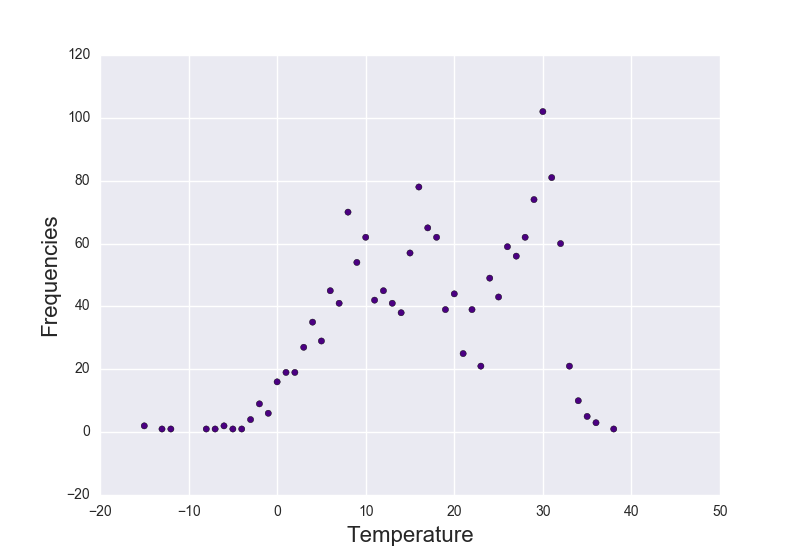
\includegraphics[width=1.0\textwidth]{tempscatt}
\end{figure}


\begin{figure}[!ht]
  \caption{The data points of temperature as categorical with range of 5}
  \centering
    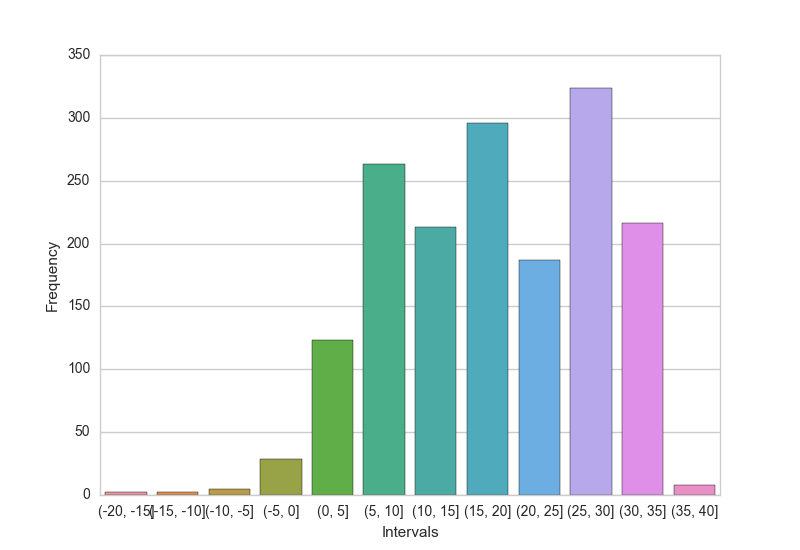
\includegraphics[width=1.0\textwidth]{range5}
\end{figure}

\begin{figure}[!ht]
  \caption{The data points of temperature as categorical with range of 10}
  \centering
    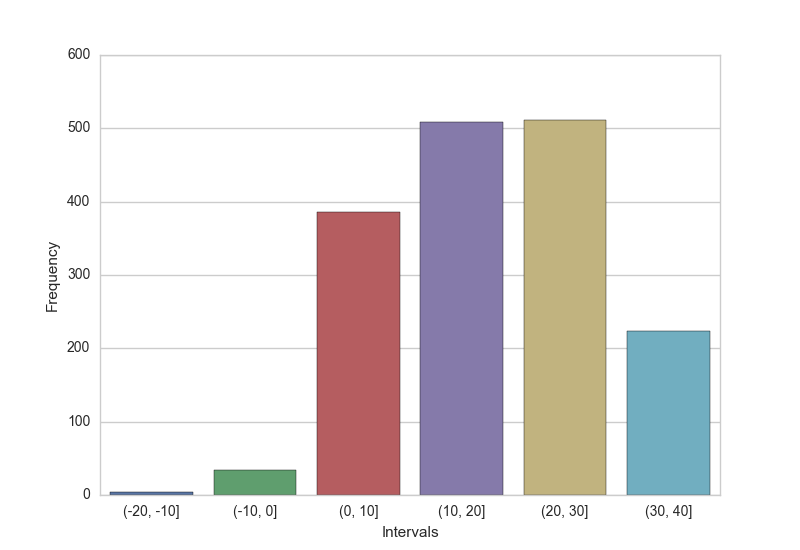
\includegraphics[width=1.0\textwidth]{range10}
\end{figure}

We also gather other numerical data that represent postal codes, data entry, building ids, and surfaces that are related to \textit{Panama papers} the international case of the shell companies \cite{panama}. The points of each sample of the different sources is plotted in figure \ref{fig:allsourcesmeans-with-outliers}. From each data source, we take 5 samples and plot them as points with the same color. We depict the mean of each source (mean of sample means and mean of standard deviation) as a triangle with the same color (the blue color is used for the temperature related dataset). We remove the outliers and plot the same data without the outliers \ref{fig:allsourcesmeans-no-outliers}. In the latter plot, there are two close clusters that are very close that they almost overlap, but this is dues to the large scale of the diagram (see figure \ref{fig:allsourcesmeans-no-outliers-zoom}).

\begin{figure}[!ht]
  \caption{The data points of the different sources (with outliers)}
  \label{fig:allsourcesmeans-with-outliers}
  \centering
    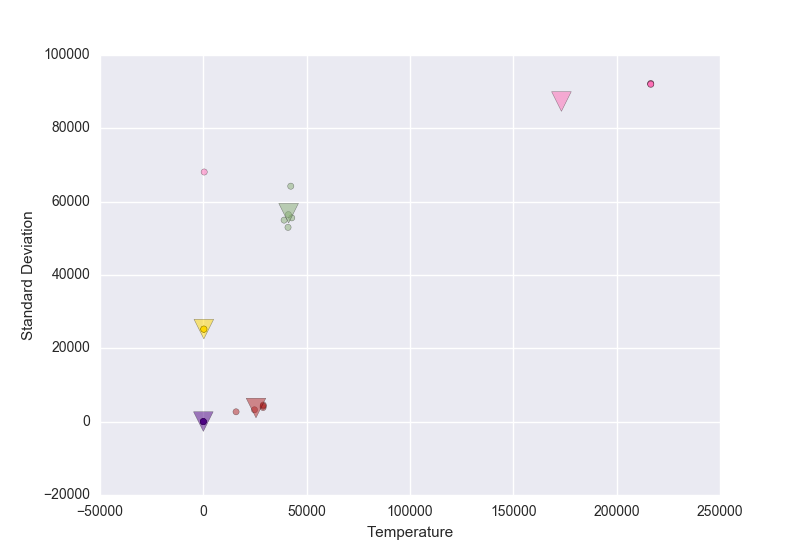
\includegraphics[width=1.0\textwidth]{allsourcesmeans_with_outliers}
\end{figure}

\begin{figure}[!ht]
  \caption{The data points of the different sources (without outliers)}
  \label{fig:allsourcesmeans-no-outliers}
  \centering
    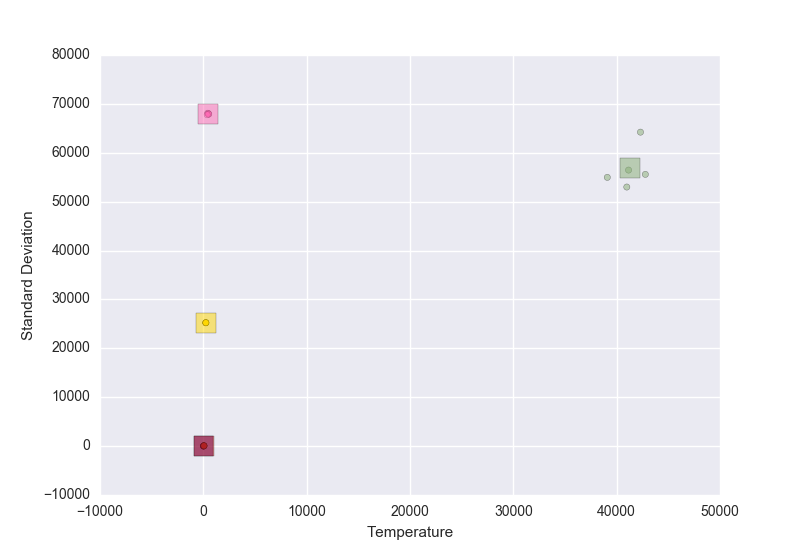
\includegraphics[width=1.0\textwidth]{allsourcesmeans_no_outliers}
\end{figure}

\begin{figure}[!ht]
  \caption{The data points of the different sources (without outliers) zoomed}
  \label{fig:allsourcesmeans-no-outliers-zoom}
  \centering
    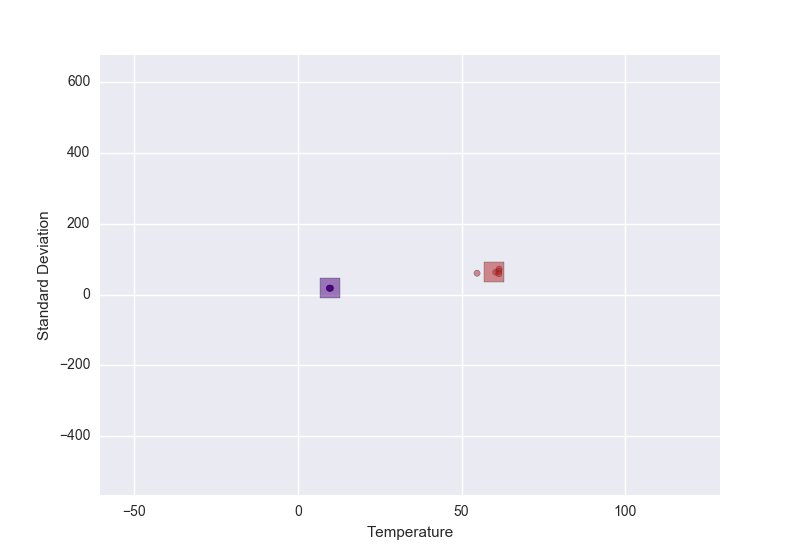
\includegraphics[width=1.0\textwidth]{allsourcesmeans_no_outliers_zoom}
\end{figure}

%\subsection{Exploratory Visualization}

\subsection{Algorithms and Techniques}


Our algorithm is influenced by \cite{unsupervised-supervised}, ``unsupervised supervised learning'' as they call it and \cite{supervised-k} ``supervised k-means'' though it is not the same.


%After the exploratory steps of the data, we dive into the machine learning core part.

We start with the data preprocessing as explain in section \ref{datapreprocessing-sec}.
%and after the data cleaning and preprocessing. 

%First part is the learning part, 
After the preprocessing, we will ends up with data as columns, each represents values for a concept's property (e.g. temperatures of cities). For each column, we divide the data into \textit{ns} samples. We have \textit{ns}=5, each sample is 20\% of the data. Next, for each sample, compute the features (see \ref{features-sec}). %As we know from the \textit{Central Limit Theorem} that the mean of samples\rq means will be approximately normal distribution. 

To reduce the dimensionality, we use \textit{Principal component analysis} (PCA). We reduce the dimensionality to 2 dimensions. After that, we cluster the samples using soft (fuzzy) clustering, namely \textit{Gaussian Mixed Model}.

Now is the second part of the algorithm, which is classifying the new data columns. We begin with the preprocessing ( e.g. removal of outliers). 

%Then, the sampling part, divide the data into the same number of samples as we did with the training data (it doesn\rq t have to be the same number \comm{Maybe I need to ignore or justify this}).

 Next, we compute the features and transform them to the reduced dimensions using PCA. Finally, calculate the belonging vector for each. The belonging vector will be a list of probabilities, each probability is corresponding to the probability of its belonging to a cluster. 
 
 
  
  %Then, calculate the belonging of each to any cluster. Since we are using soft clustering, the belonging is a vector of probabilities, each is corresponding to a specific cluster.

%We then Calculate the probability for each sample the belong to  to any of the clusters. Since we are using soft clustering, each of the points may belong to multiple clusters each with a probability between 0 and 1.


%We will be performing statistical tests for each column in for each dataset. Then, we will reduce the dimensionality using PCA. After the dimensionality reduction, we use soft (fuzzy) clustering, more specifically \comm{Gaussian Mixture Model} \comm{reference}. This will result in each column in the data sets to be presented in a point in an n-dimensional space and located in a cluster.  \comm{reference soft clustering} 

%Next, we do supervised machine learning. We have the new features, and we have for each point, the clusters it belongs to with the percentage.


\subsubsection{features} \label{features-sec}
Here are using the mean and standard deviation. But will be using the following statistical tests:
\begin{itemize}
\item Kolmogorov–Smirnov test
\item Anderson–Darling test
\item Jarque–Bera test
%\item Goodness of fit
\item Cramér–von Mises criterion
\item Akaike information criterion
\item Hosmer–Lemeshow test
\item Shapiro–Wilk test
\item Kuiper's test
\item Coefficient of determination R\^{}2
\item Mann–Whitney U test
\item Wilcoxon signed-rank test
\item Sign test
\item Kruskal–Wallis one-way analysis of variance
%One-way analysis of variance
\item Friedman test
\item Kendall's W
\item Jonckheere's trend test
\item $r^2$ correlation $ r^2 = \frac{t^2}{t^2 + df} $
\end{itemize}

\subsection{Benchmark}\label{benchmark-sec}
According to our knowledge, there is no agreed upon benchmark in the literature. We think that is due to different variation of the problem. For example this paper \cite{karma}, does not distinguish between numerical, textual or categorical data in the evaluation. This paper on the other hand \cite{ann-ser-webtables} the authors do not have the training and testing data disjoint. They justified it with the large number features used and that they did not notice overfitting. In the latter paper, the authors used F1 as the metric, and they reported the Wiki Manual with F1 score 56.12 and Web Manual with 43.23 as the F1 score. Wiki Manual and Web Manual are tables extracted from Wikipedia with the former has less noisy data than the other \cite{ann-ser-webtables}.



\section{Methodology (3-5 pages)}
We will be using quantitative research methodology in our work and compare it to the benchmark mentioned in section \ref{benchmark-sec}. %We will compare the precision and recall with the same data.

\subsection{Data Preprocessing} \label{datapreprocessing-sec}



There are two sources of data that we will be using for the learning process, the first source is a SPARQL endpoint \cite{w3c-sparql} (we use DBpedia) and the second data source is a csv file (we can use excel or pdf as well). 

For the SPARQL endpoint, we query the endpoint to get the data as tabular format to apply the statistical tests and compare it with the second source. For every concept and property of interest,% So we query every concept that we have in the mapping file \comm{I should explain it or add a reference to it} 
we use SPARQL with the \textit{concept} and \textit{subject} as strings (e.g. for the concept to be ``\textless http://schema.org/City\textgreater '' and for the subject to be ``\textless http://dbpedia.org/property/novHighC\textgreater'')(see figure \ref{fig:sparql-sk} and \ref{fig:sparql-example}). We use \cite{loupe} to find concepts and their properties as explained in the data exploration section. After that, we have each property of a concept as a column of data, so we save it as csv file.

For the second data source, if it was not in csv file, we convert it to csv format. This is straight forward step as we are assuming the second data source to be in a tabular form. 

After having the data for the two sources, we remove the outliers from both of them using \textit{Tukey\rq s} method. It is basically removing values that are less than 1.5 of the difference between the 25th percentile and 75th percentile subtracted from the 25th percentile or added to the 75th percentile. 
$$ outliers < [25th percentile - ( ( 75th percentile - 25th percentile )*1.5)] $$
$$ [ 75th percentile + ( ( 75th percentile - 25th percentile )*1.5)] < outliers  $$

In figure \ref{fig:allsourcesmeans-with-outliers} the outliers for the pink dataset is clearly affect the mean of the pink cluster. After applying \textit{Tukey\rq s} method, the mean of the cluster is shifted dramatically to the left, which means the that outliers where pulling it to the right direction.

\begin{figure}
  \caption{SPARQL Query Skeleton}
  \label{fig:sparql-sk}
\begin{lstlisting}[language=SPARQL]
SELECT ?object where {
        ?x a <Concept> .
        ?x  <Subject> ?object .
        }
\end{lstlisting}
\end{figure}

\begin{figure}
  \caption{SPARQL Query Example}
  \label{fig:sparql-example}
\begin{lstlisting}[language=SPARQL]
SELECT ?object where {
        ?x a <http://schema.org/City> .
        ?x  <http://dbpedia.org/property/novHighC> ?object .
        }
\end{lstlisting}
\end{figure}


\subsection{Implementation}
\subsection{Refinement}


\section{Results (2-3 pages)}
\subsection{Model Evaluation and Validation}
\subsection{Justification}

\section{Conclusion (1-2 pages)}
 \subsection{Free-Form Visualization}
 \subsection{Reflection}
 \subsection{Improvement}
 
 
\begin{thebibliography}{99}

\bibitem{webtables-power-2008}Cafarella, Michael J., et al. "Webtables: exploring the power of tables on the web." Proceedings of the VLDB Endowment 1.1 (2008): 538-549.

\bibitem{unsupervised-supervised}
Balasubramanian, Krishnakumar, Pinar Donmez, and Guy Lebanon. "Unsupervised supervised learning II: Margin-based classification without labels." Journal of Machine Learning Research 12.Nov (2011): 3119-3145.

\bibitem{karma}
Taheriyan, Mohsen, et al. "A scalable approach to learn semantic models of structured sources." Semantic Computing (ICSC), 2014 IEEE International Conference on. IEEE, 2014.

\bibitem{ann-ser-webtables}
Limaye, Girija, Sunita Sarawagi, and Soumen Chakrabarti. "Annotating and searching web tables using entities, types and relationships." Proceedings of the VLDB Endowment 3.1-2 (2010): 1338-1347.

\bibitem{dbpedia-site}
http://wiki.dbpedia.org/

\bibitem{w3c-sparql}
https://www.w3.org/wiki/SPARQL

\bibitem{loupe}
http://loupe.linkeddata.es/

\bibitem{panama}
https://offshoreleaks.icij.org/pages/database

\bibitem{supervised-k}
Finley, Thomas, and Thorsten Joachims. "Supervised k-means clustering." (2008).














\end{thebibliography}
\end{document}








